\documentclass{article}
\usepackage[margin=1.0in]{geometry}
\usepackage{amsmath}
\usepackage{graphicx}
\usepackage{cite}
\usepackage[hidelinks]{attachfile}
\usepackage{mwe}
\newcommand{\cen}[1]{\begin{equation}\ce{#1}\end{equation}}
% \usepackage{subcaption}
% \usepackage{caption}
\usepackage{csvsimple,booktabs}
\usepackage{navigator}
\usepackage{hyperref}
\usepackage{caption,subfigure}
\usepackage{textcomp}
\usepackage{epsf}
\usepackage{bm}
\usepackage{setspace}
\usepackage{caption,subfigure}

% \setcounter{secnumdepth}{0}
%----------------------------------------------------------------------------------------
%	NAME AND CLASS SECTION
%----------------------------------------------------------------------------------------

\newcommand{\preTitle}{Final\ Project Report}
\newcommand{\hmwkTitle}{Using Machine Learning to Estimate Energy Performance of Residential Buildings} % title
\newcommand{\hmwkDueDate}{Wednesday,\ December\ 3,\ 2019} % Due date
\newcommand{\hmwkClass}{DATA\ 1030} % Course/class
\newcommand{\hmwkClassTime}{TTh 1pm-2:20pm} % Class/lecture time
\newcommand{\hmwkClassInstructor}{Doc.\ Andras\ Zsom} % Teacher/lecturer
\newcommand{\hmwkAuthorName}{Cheng Zeng} % Your name
%\usepackage[a4paper, body={16.8cm, 23cm}]{geometry}
\setlength\parindent{0pt}

%----------------------------------------------------------------------------------------
%	TITLE PAGE
%----------------------------------------------------------------------------------------
\title{
\vspace{2in}
\textmd{\hmwkClass:\ \preTitle \\ \textbf{\hmwkTitle}}\\
\normalsize\vspace{0.1in}\small{Due\ on\ \hmwkDueDate}\\
\vspace{0.1in}\large{\textit{\hmwkClassInstructor}}\\
\vspace{0.1in}\large{\hmwkClassTime}
\vspace{3in}
}

\author{\vspace{0.2in} \textbf{\hmwkAuthorName} \\
School of Engineering, Brown University} 

\date{\today } % Insert date here if you want it to appear below your name
%----------------------------------------------------------------------------------------

\begin{document}

\maketitle

\hfil github: \href{https://github.com/cengc13/DATA1030_final_project}{https://github.com/cengc13/DATA1030\_final\_project} \par.

\setlength{\parskip}{1em}

\section{Introduction \label{sec:intro}}
\subsection{Motivation}
This final project aims to understand the energy efficiency of residential buildings. Given eight attributes of a given, there are two variables named \textbf{heating load} and \textbf{cooling load} characterizing the energy efficiency. Since the outputs are continuous variables. It is essentially a regression problem. It is important because it could help to design environmentally friendly buildings from the theoretical perspective.  On-site experiments could be intractable, time and effort consuming. 


\subsection{Dataset}
This dataset originates from the \href{https://archive.ics.uci.edu/ml/datasets/Energy+efficiency}{UCI energy efficiency}. It has $\mathbf{768}$ simulation points. Each point has ten features, including $8$ input features and $2$ target features. No missing values exist for this dataset. In Table.~\ref{tab:feature}, following the classical mathematical convention, X denotes input variables whereas Y denotes target variables. To make it more clear, the exact meaning of the two target variables are elaborated.

\begin{enumerate}
	\item[\bullet] heating load: the amount of heat energy that would need to be added to a space to maintain the temperature in an acceptable range.

	\item[\bullet] cooling load: the amount of heat energy that would need to be removed from a space (cooling) to maintain the temperature in an acceptable range.
\end{enumerate}

\begin{table}[!htbp]
\centering 
\captionsetup{font=footnotesize}
\caption{Input and output variables.}
 \begin{tabular}{*{4}c}
\hline \hline
Math symbols & Input/Output variable & possible values &  units/description \\
\hline
$X1 $ & Relative compactness &   $12$ & absolute unit   \\
$X2$ & Surface area & $12$ &  m$^2$ \\
$X3$  &  Wall area  &   $7$ &  m$^2$   \\
$X4$  &  Roof area  &   $4$ &  m$^2$   \\
$X5$  &  Overall height  &   $2$ &  m   \\
$X6$  &  Orientation  &   $4$ &  2:North, 3:East, 4:South, 5:West   \\
$X7$  &  Glazing area  &   $4$ &  $0\%$, $10\%$, $25\%$, $40\%$ (of floor area)   \\
$X8$  &  Glazing area distribution  &   $5$ &  0:Unknow, 1:Uniform, 2:North, 3:East, 4:South, 5:West   \\
$Y1$  &  Heating load  &   $586$ &  kWh/m$^2$   \\
$Y2$  &  Cooling load  &   $636$ &  kWh/m$^2$   \\
\hline \hline
\end{tabular}
\label{tab:feature}
\end{table}


\section{Exploratory Data Analysis \label{sec:eda}}

We first investigate the properties of two target variables. Fig.~\ref{fig:heating_load} and Fig.~\ref{fig:cooling_load}. As one can see, the two target variables do not follow a simple distribution such as normal distribution. Also, we can see that the two target variables have similar shape of distribution. It indicates that a building with high heating load may also display cooling load.


\begin{figure}[!bht]
\centering     \captionsetup{font=footnotesize, width=.6\textwidth}
\subfigure[Heating load]{
  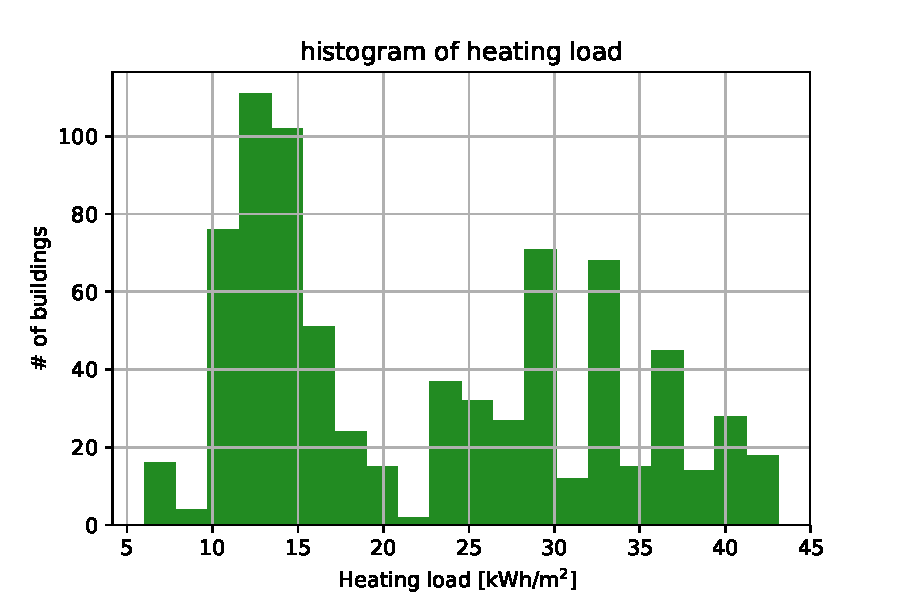
\includegraphics[scale=0.40]{../../figures/Y1_hist.pdf}
  \label{fig:heating_load}}
% \quad
\subfigure[Cooling load]{
  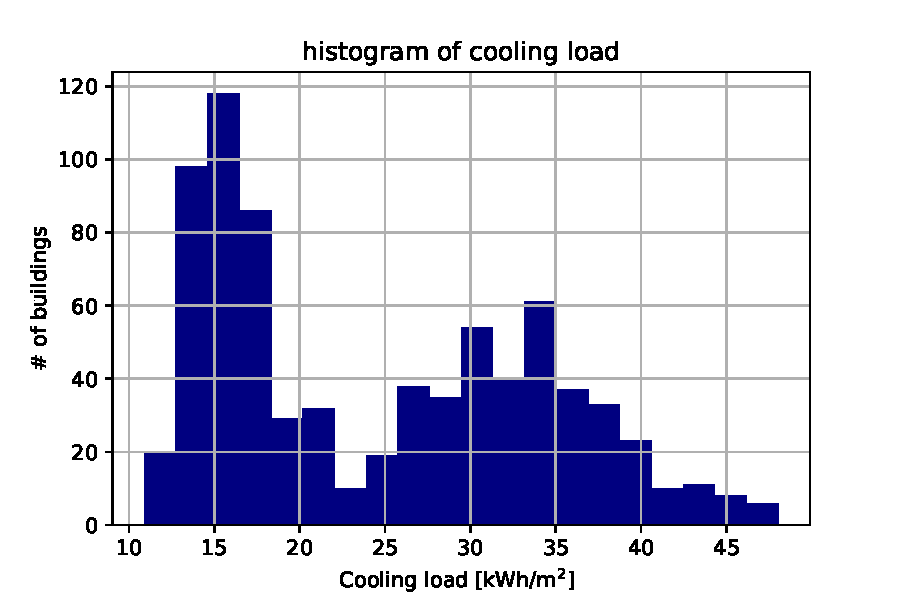
\includegraphics[scale=0.40]{../../figures/Y2_hist.pdf}
 % \subcaption{Normal mode 2}
  \label{fig:cooling_load} }
\caption{Properties of two target variables} 
\end{figure}

The Fig.~\ref{fig:heating_load_versus_continuous} and Fig.~\ref{fig:cooling_load_versus_continuous} indicate that the relationship between the input variables and target variable is not trivial. It suggests that a simpler learner such as linear regression is not able to describe this complicated behavior, we need more sophisticated model such as random forest regression to justify this relationship.


\begin{figure}[!bht]
\centering     \captionsetup{font=footnotesize, width=.6\textwidth}
\subfigure[Heating load versus continuous features]{
  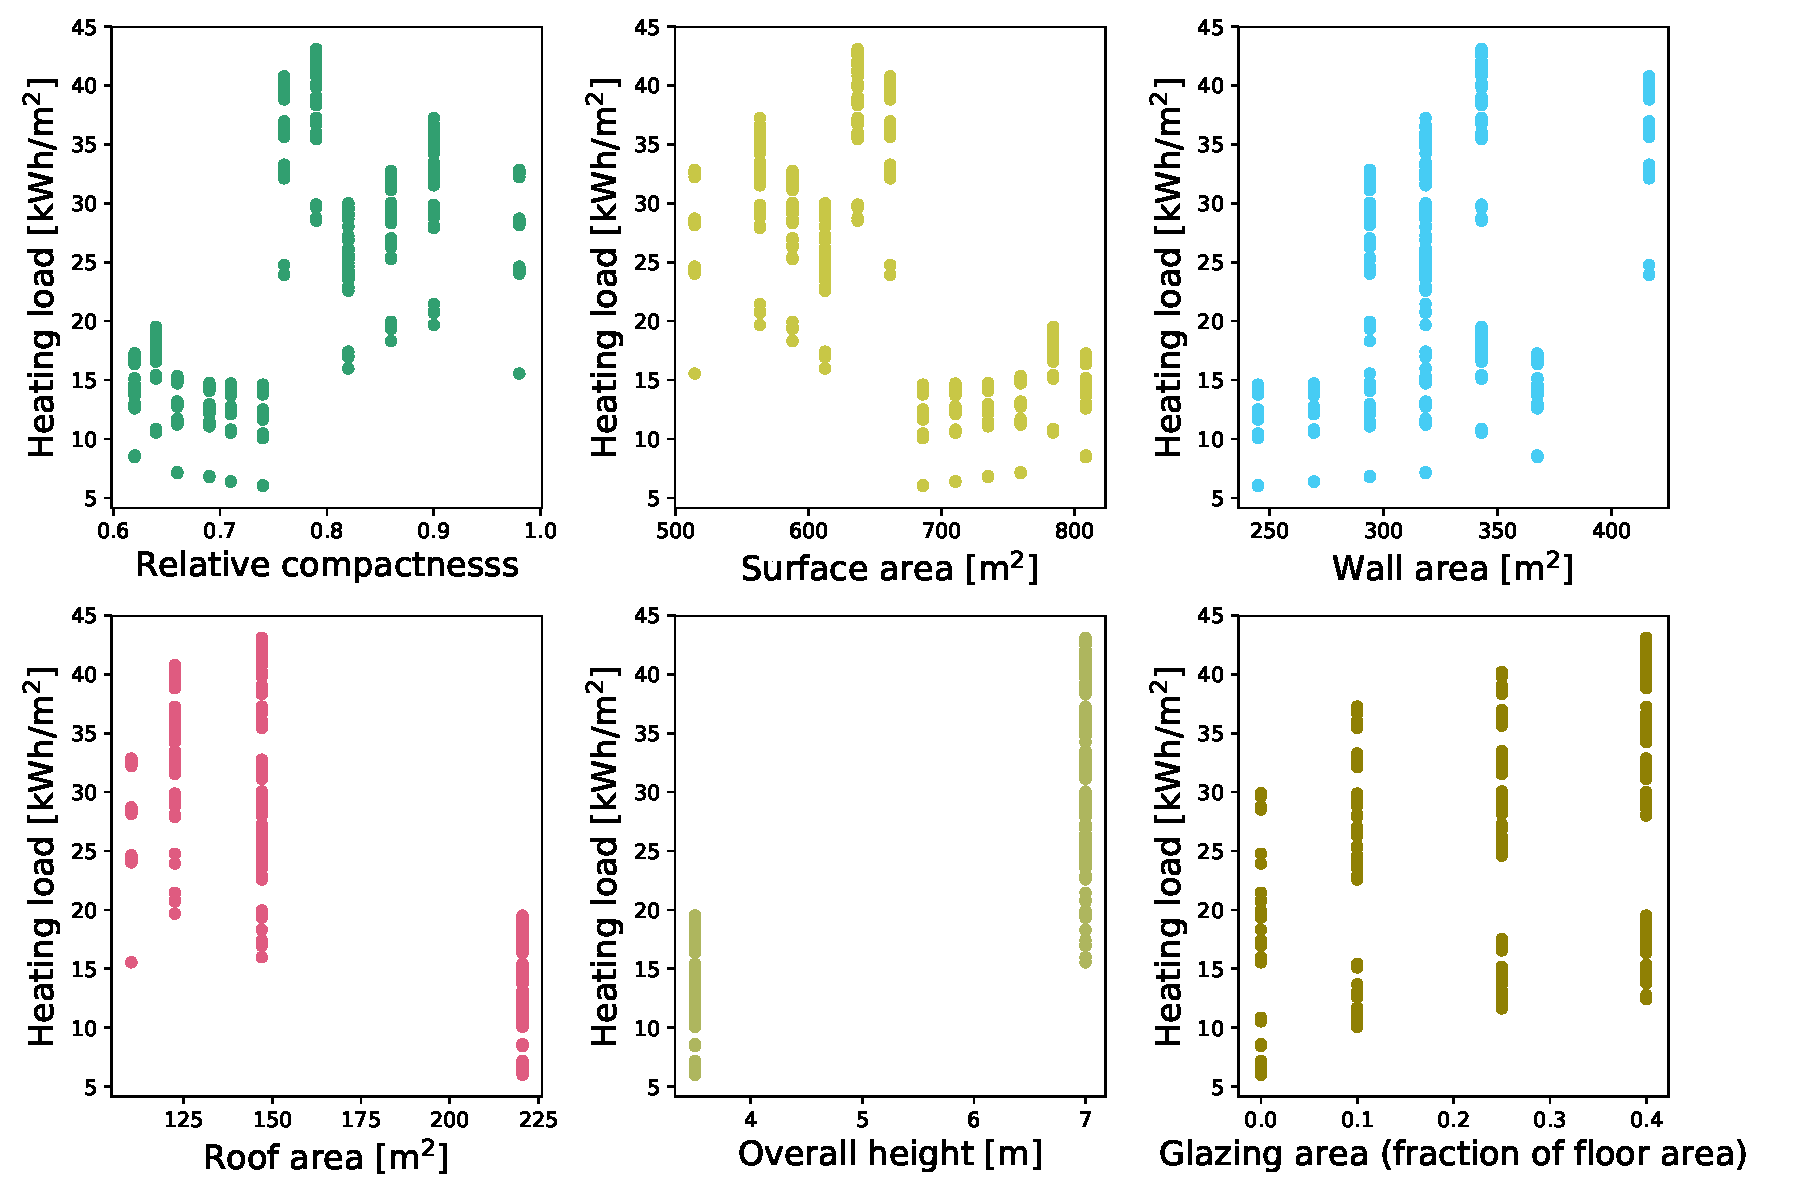
\includegraphics[scale=0.40]{../../figures/Y1_vs_continuous_features.pdf}
  \label{fig:heating_load_versus_continuous}}
% \quad
\subfigure[Cooling load versus continuous features]{
  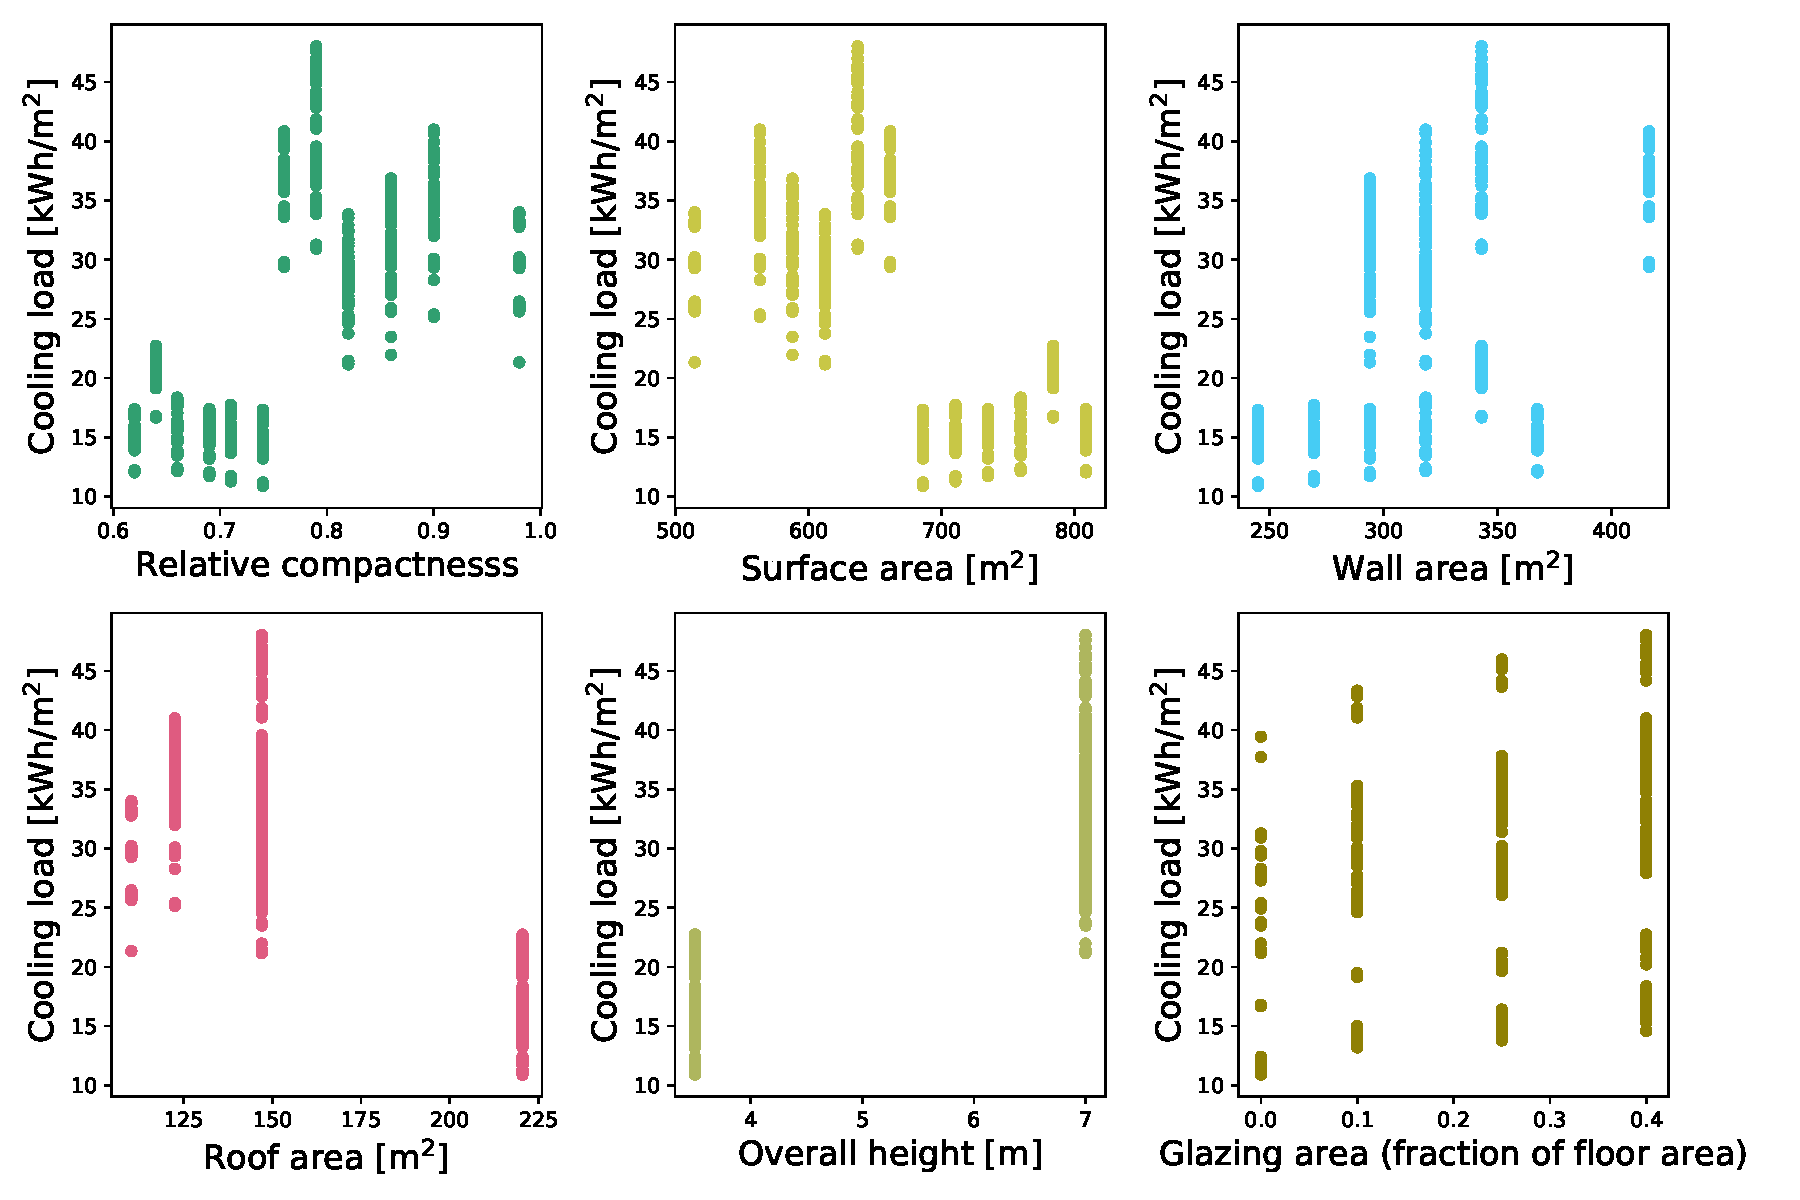
\includegraphics[scale=0.40]{../../figures/Y2_vs_continuous_features.pdf}
 % \subcaption{Normal mode 2}
  \label{fig:cooling_load_versus_continuous} }
\caption{Interaction of two target variables with continuous features} 
\end{figure}

% \vspace{0.1in}
The Fig.~\ref{fig:heating_load_versus_categorical} and Fig.~\ref{fig:cooling_load_versus_categorical} indicate that the relationship between the input variables and target variable is not trivial. It suggests that a simpler learner such as linear regression is not able to describe this complicated behavior, we need more sophisticated model such as random forest regressor to justify this relationship.

\begin{figure}[!bht]
\centering     \captionsetup{font=footnotesize, width=.6\textwidth}
\subfigure[Heating load versus categorical features]{
  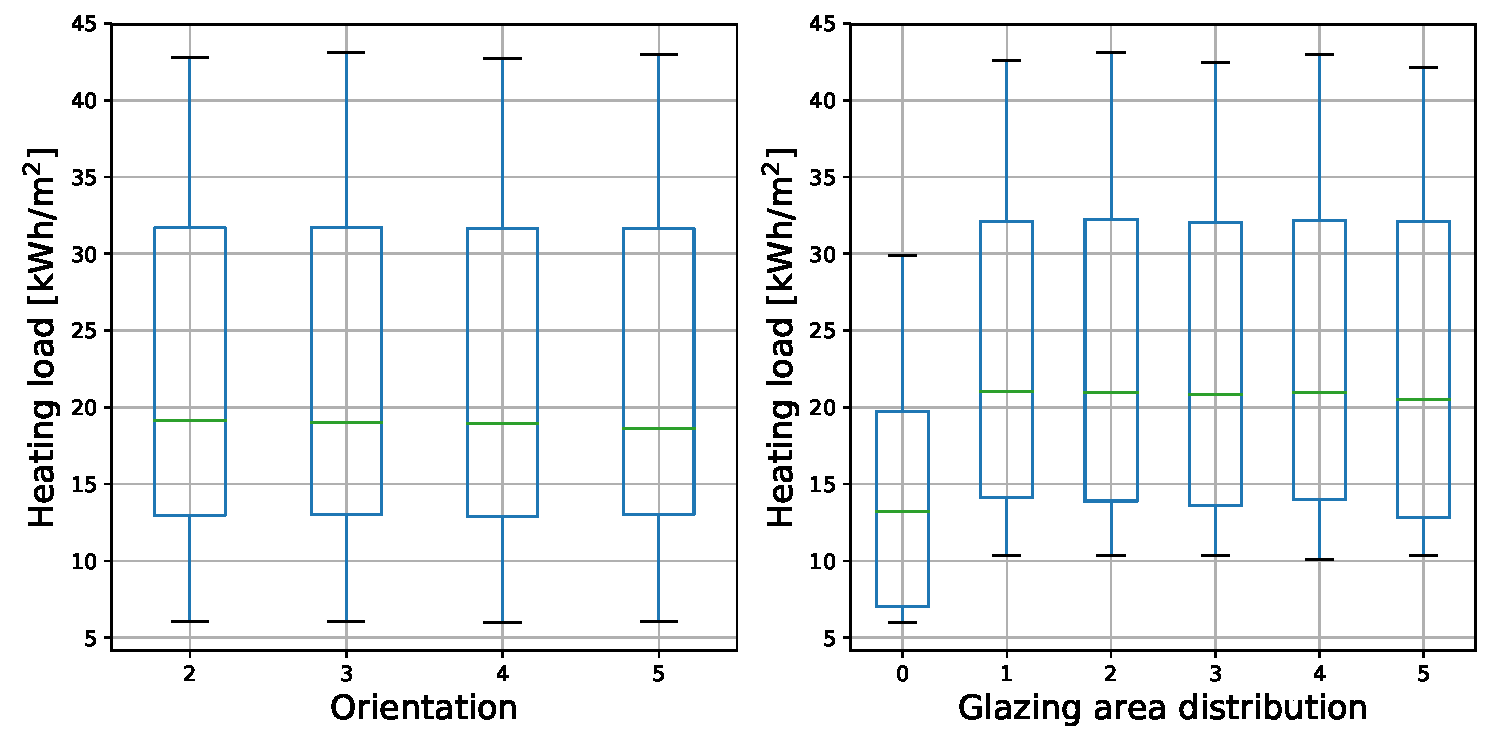
\includegraphics[scale=0.40]{../../figures/Y1_vs_categorical_features.pdf}
  \label{fig:heating_load_versus_categorical}}
% \quad
\subfigure[Cooling load versus categorical features]{
  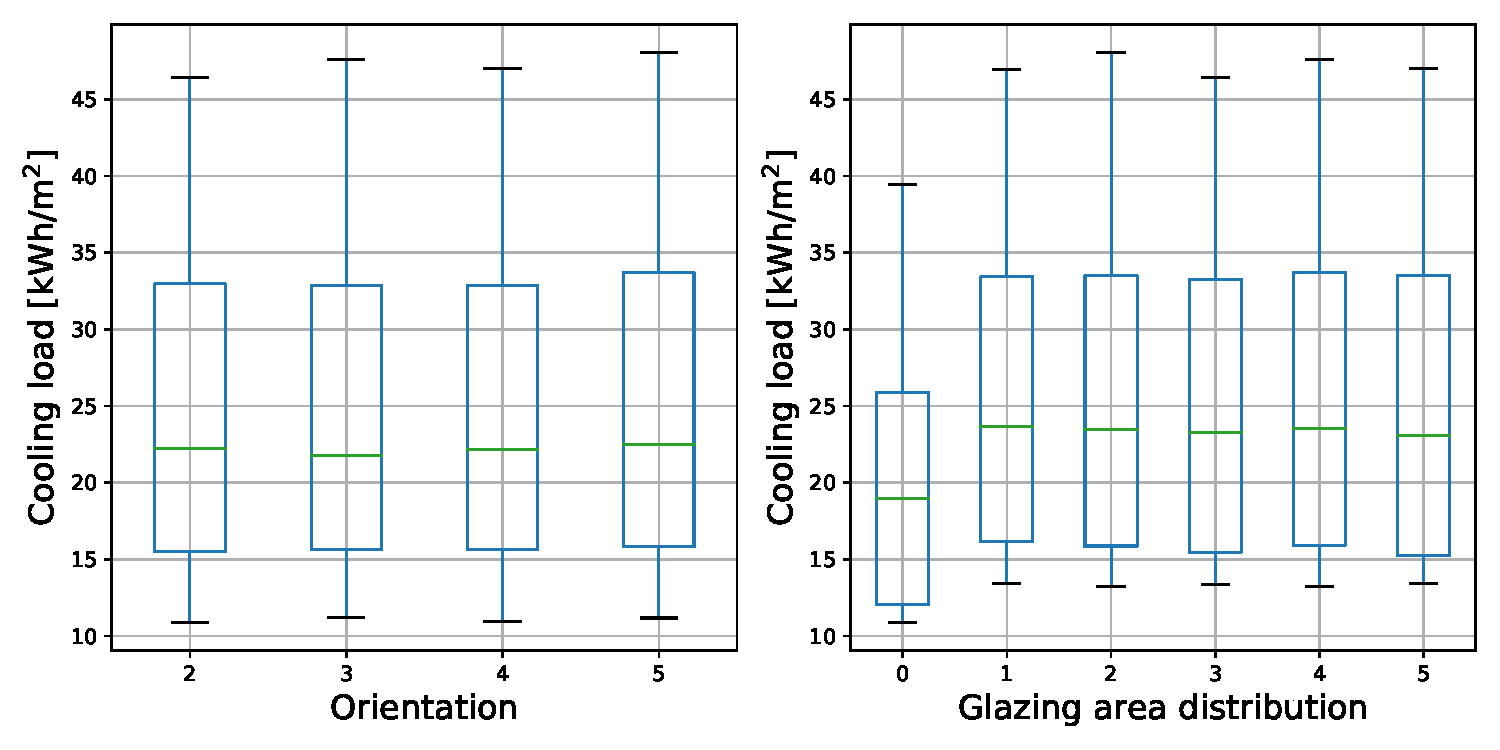
\includegraphics[scale=0.40]{../../figures/Y2_vs_categorical_features.pdf}
 % \subcaption{Normal mode 2}
  \label{fig:cooling_load_versus_categorical} }
\caption{Interaction of two target variables with categorical features} 
\end{figure}


We compute the correlation matrices for both target variables and rand with the absolute variables with respect to the target variable. In Fig.~\ref{fig:heating_load_corr} and Fig.~\ref{fig:cooling_load_corr} implies that overall height (X5), roof area (X4), surface area (X2) and 
compactness (X1) show the highest linear correlation with both target variables.

\begin{figure}[!bht]
\centering     \captionsetup{font=footnotesize, width=.6\textwidth}
\subfigure[Correlation matrix for heating load]{
  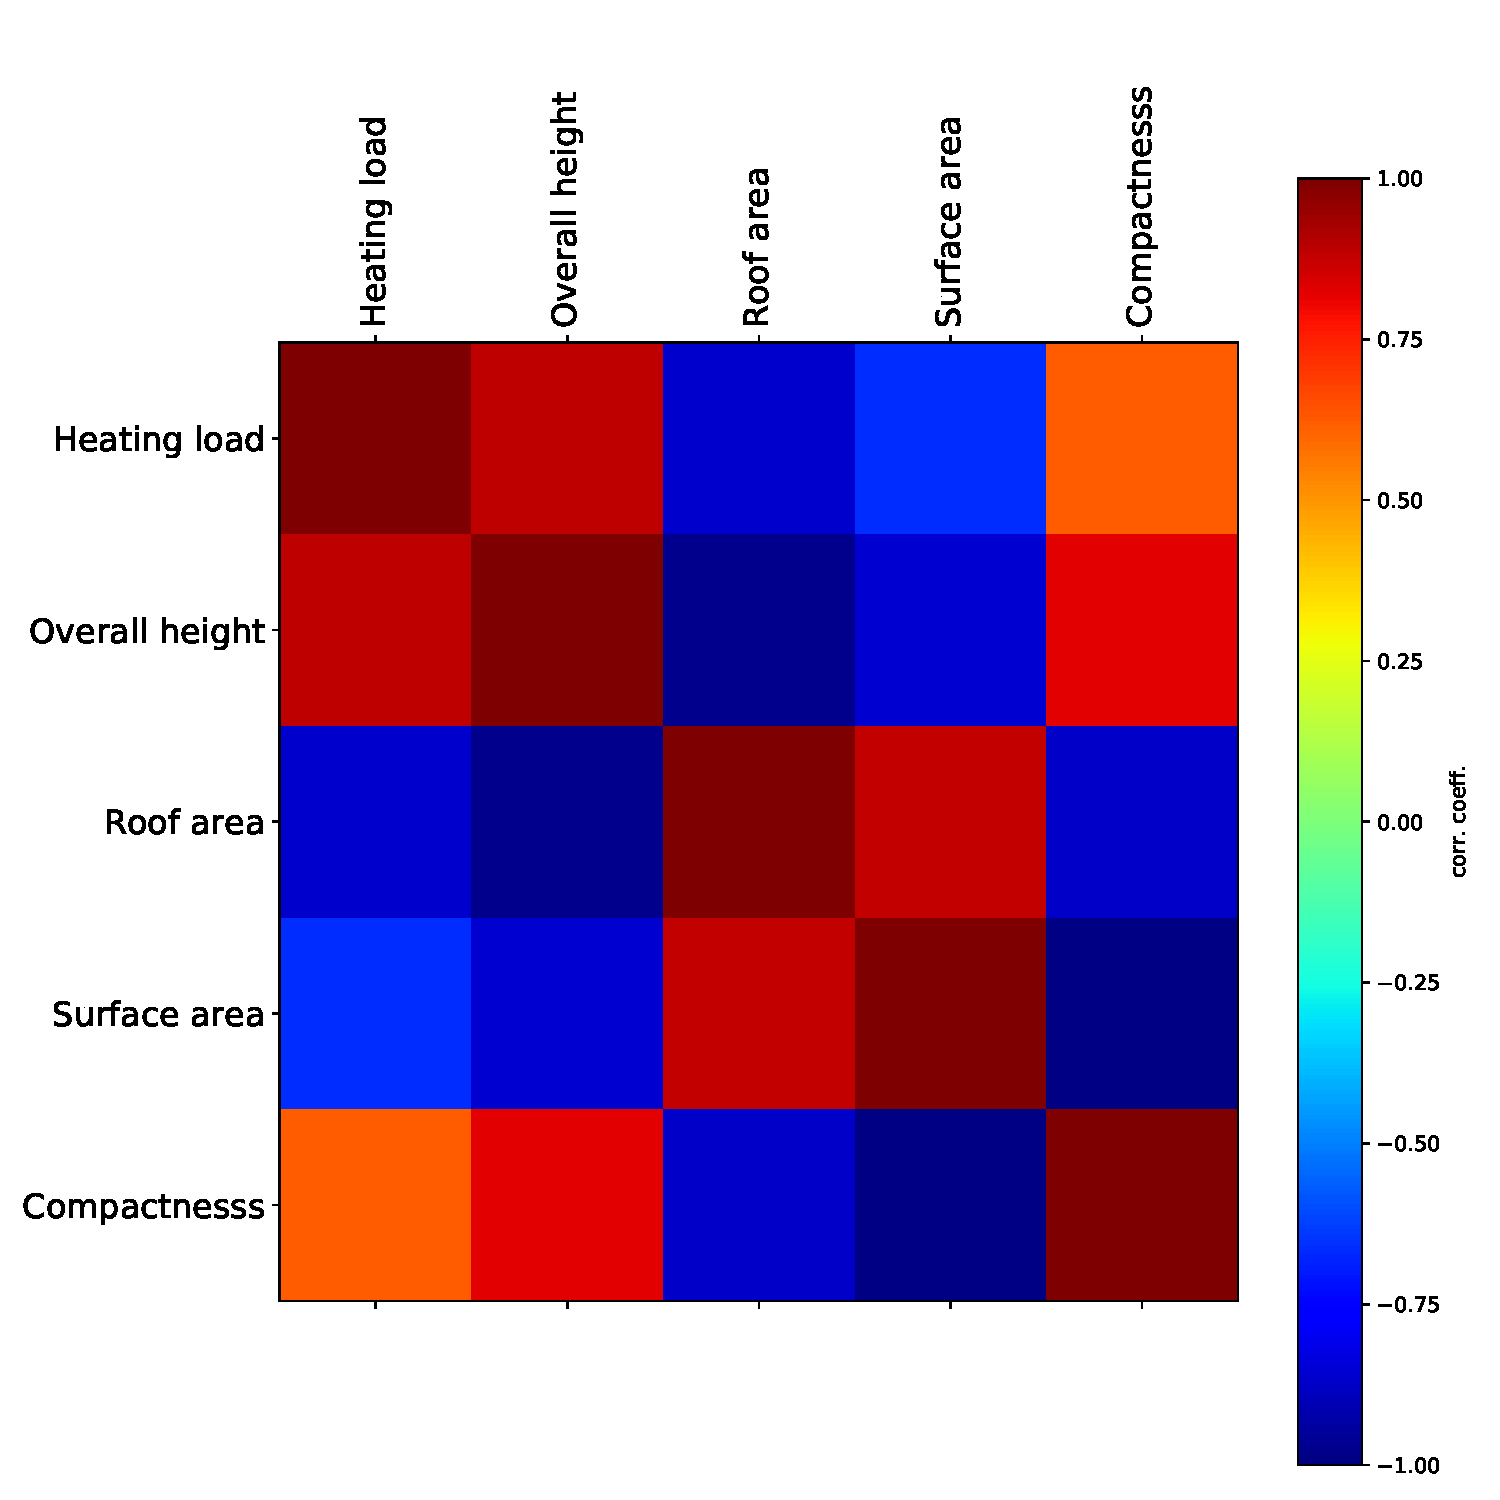
\includegraphics[scale=0.30]{../../figures/corrmat_on_Y1-sorted.pdf}
  \label{fig:heating_load_corr}}
% \quad
\subfigure[Correlation matrix for cooling load]{
  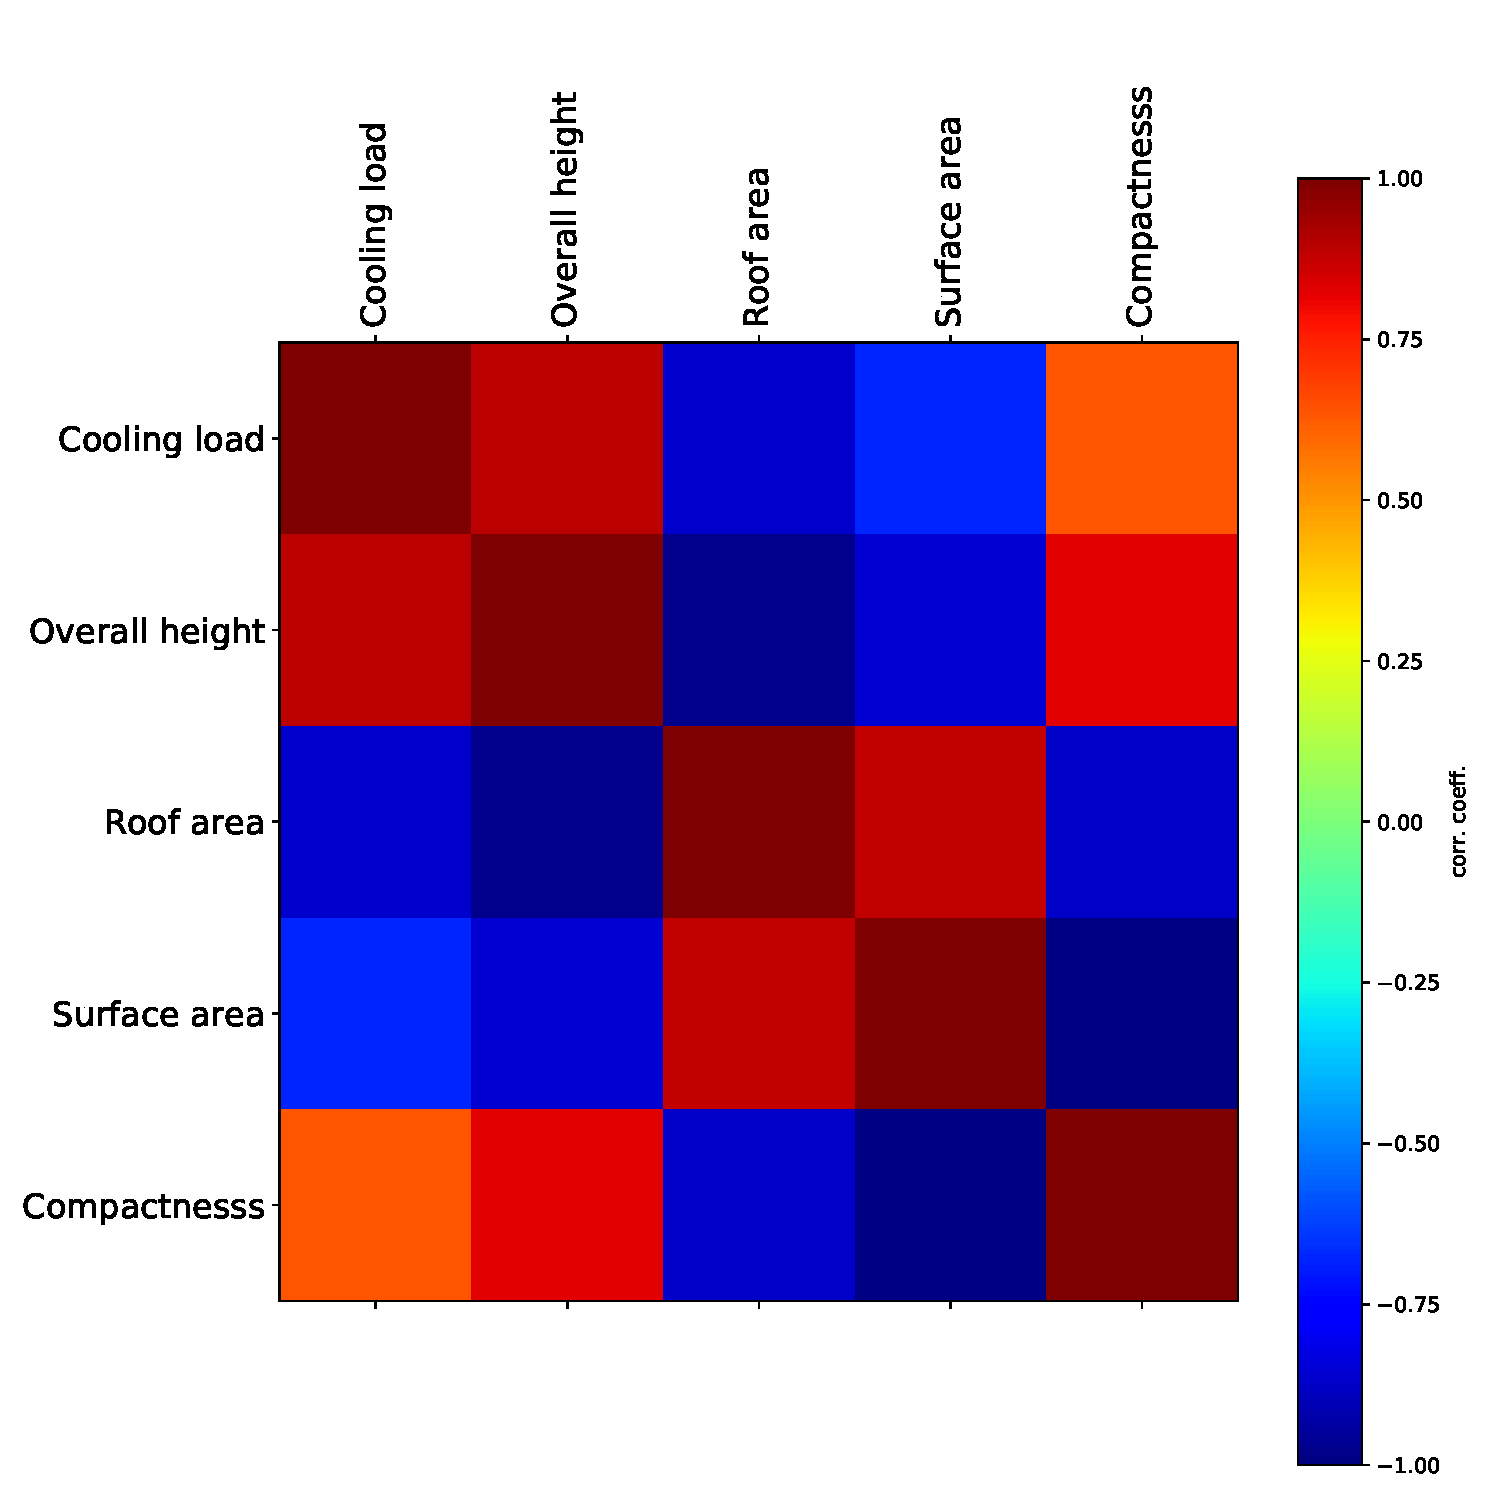
\includegraphics[scale=0.30]{../../figures/corrmat_on_Y2-sorted.pdf}
  \label{fig:cooling_load_corr} }
\caption{Correlation matrices} 
\end{figure}


\section{Methods \label{sec:methods}}
\subsection{Preprocessing}
We elaborate on the preprocessing for various types of features

\begin{enumerate}
	\item[\bullet] Six continuous features (X1, X2, X3, X4, X5 and X7): since all the features are well bounded. \textit{MinMaxScaler} is applied. 

	\item[\bullet] Two categorical features (X6 and X8): one-hot encoding is used because the categories cannot be ordered.

	\item[\bullet] target variables (Y1 and Y2): in terms of the regression problem, it is kept as it is. 
\end{enumerate}
After preprocessing, there are in total $16$ input features and $2$ output features.

\subsection{Machine learning pipeline}
The following discussion applies to pipelines of models for both target variables. I used the ordinary k fold cross-validation (CV) because the dataset is identically and independently distributed.
Five folds are used. The data splits to three parts ($64\%$ train, $16\%$ CV, $20\%$ test). The dataset is shuffled before splitting with given random state to make sure that this process is reproducible. Ten different random states  are used to estimate the uncertainties  due to data splitting. For non-deterministic methods, the uncertainty for the model itself is evaluated by fixing the random state for data splitting while varying the random state for the model for $5$ times. I tried four machine learning methods and tuned the hyperparameters using a grid search.

For linear regression model, I used \textit{Lasso} linear model and I tuned the regularization strength (alpha values) in the range between $0.0001$ and $100$.
For random forest, the maximum depth and minimum samples for a split are tuned. I tried the range of $2$ to $20$ for maximum depth and the range of 2 to 12 for minimum samples for a split. 
For Support vector regression, I tuned the C and gamma, trying the range of 
$1$ to $1000$, and $0.0001$ to $100$, respectively. 
For multilayer perceptron regression, I tuned the regularization coefficients (alpha) in the range of 0.0001 to 0.01, and the number of nodes in hidden layers (I tied 10 and 15 nodes). 

For the metrics, I used both mean squared error (MSE) and R2 score to evaluate the model performance. MSE is the typical metric used for evaluating a regression model. R2 score is useful when it comes to evaluating the feature importance, especially in comparison of the baseline model whose R2 score is supposed to be $0$.

\subsection{Results}
The R2 score given by a baseline model that predicts the mean of $y$ is $0$.
In table.~\ref{tab:results_heating_load} and  table.~\ref{tab:results_cooling_load}, we show the MSE and R2 score of prediction on the testing set for heating load and cooling load respectively. Values following $\pm$ indicate the uncertainties due to data splitting. Values in the bracket are the uncertainties due to non-deterministic models, for which only results using MSE metric are evaluated. 

\begin{table}[!htbp]
\centering 
\captionsetup{font=footnotesize}
\caption{The test MSE and R2 score for heating load (Y1)}
 \begin{tabular}{*{3}c}
\hline \hline
Methods & Test MSE & R2 score  \\
\hline
Lasso Linear Model & $7.938 \pm 0.658$ &   $0.923 \pm 0.005$   \\
Random Forest & $0.283 \pm 0.037 (0.009)$ & $0.997 \pm 0.0003$ \\
Support Vector Machine  &  $6.650 \pm 0.693$  &   $0.936 \pm 0.004$   \\
Multilayer Perceptron Regression  &  $0.344\pm0.071 (3.541)$  &   $0.997 \pm 0.001$   \\
\hline \hline
\end{tabular}
\label{tab:results_heating_load}
\end{table}

\begin{table}[!htbp]
\centering 
\captionsetup{font=footnotesize}
\caption{The test MSE and R2 score for cooling load (Y2)}
 \begin{tabular}{*{3}c}
\hline \hline
Methods & Test MSE & R2 score  \\
\hline
Lasso Linear Model & $10.044 \pm 1.183$ &   $0.890 \pm 0.007$   \\
Random Forest & $3.317 \pm 0.426 (0.233)$ & $0.964 \pm 0.003$ \\
Support Vector Machine  &  $10.082 \pm 1.625$  &   $0.890 \pm 0.012$   \\
Multilayer Perceptron Regression  &  $2.386\pm0.625 (2.836)$  &   $0.997 \pm 0.001$   \\
\hline \hline
\end{tabular}
\label{tab:results_cooling_load}
\end{table}

Among all the models studied, Random Forest is the best one for target variable of heating load (Y1), with MSE of R2 score as $0.283$ and $0.997$, respectively. For cooling load, multilayer perceptron regression (neural network) is the  best model, with MSE and  R2 score as $2.386$ and $0.997$, respectively. It is consistent with the finding from Fig.~\ref{fig:cooling_load_versus_continuous} that a complicated learner is needed to justify the curvy correlation between input variables and output variables.
Another interesting observation is that heating load can be estimated much more accurately that cooling load, which might suggest that some input variables are more strongly associated the heating load. In terms of the uncertainties, in brief the more accurate the model is, the lower the uncertainty due to data splitting will be. However, for the neural network regressor, the uncertainty due to the model itself is very large compared to the other non-deterministic model, Random Forest. 

\subsection{Global feature importance \label{subsec:gfi}}
We note that there is a large model uncertainty for neural network regression. For the feature importance analysis, we will focus on the random forest model, which gives more stable and consistent performance. We will use R2 score as the metric for feature importance evaluation. 

We determine the global feature importance by a permutation test. We found that relative compactness is the most important feature for both output variables (see Fig.~\ref{fig:permutation_Y1} and Fig.~\ref{fig:permutation_Y2}). It makes sense because it defines the surface-to-volume of the building, which is an important properties for heat transfer. Interesting, the second most important feature is the glazing area (X7), that does not show up in the simple linear correlation analysis. From engineering perspective, it is intuitively understood that glazing area is of great importance because the amount of glazing is associated with the heat adsorbed from the sun. It implies that statistical learning has potential in mining  hidden pattern behind the data. The results fit into a human/academic context because it agrees with our common sense. For example, it is well-acknowledged in scientific community that relative compactness is an important factor related to the energy efficiency of buildings. I also studies the global feature importance using \textit{Shapley}, the results are shown in Fig.~\ref{fig:shap_Y1} and Fig.~\ref{fig:shap_Y2}, and it is mostly consistent with permutation test despite that 
the order of importance of features for heating load is now slightly different than that for cooling load.

\begin{figure}[!bht]
\centering     \captionsetup{font=footnotesize, width=.6\textwidth}
\subfigure[Permutation test for heating load]{
  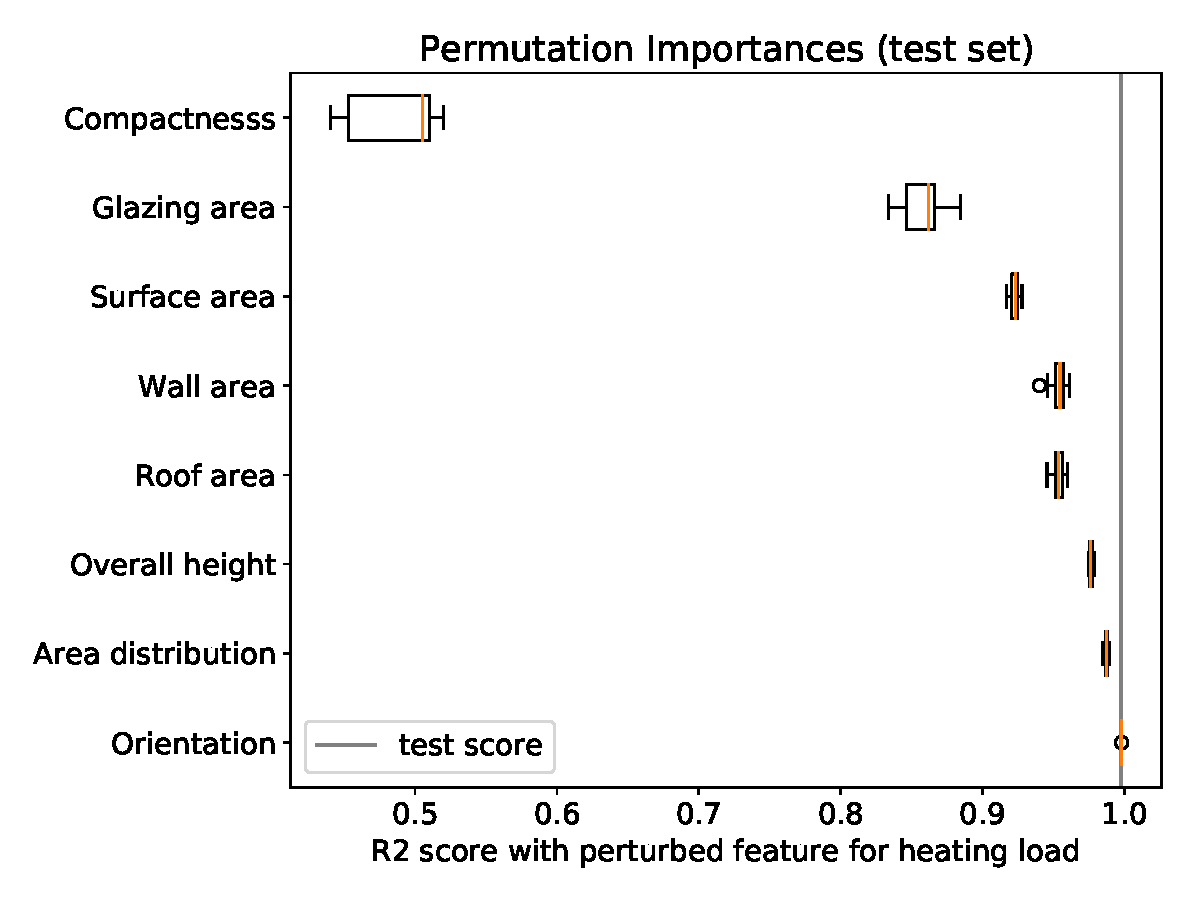
\includegraphics[scale=0.38]{../../figures/Y1_gfi_permutation.pdf}
  \label{fig:permutation_Y1}}
% \quad
\subfigure[Permutation test for cooling load]{
  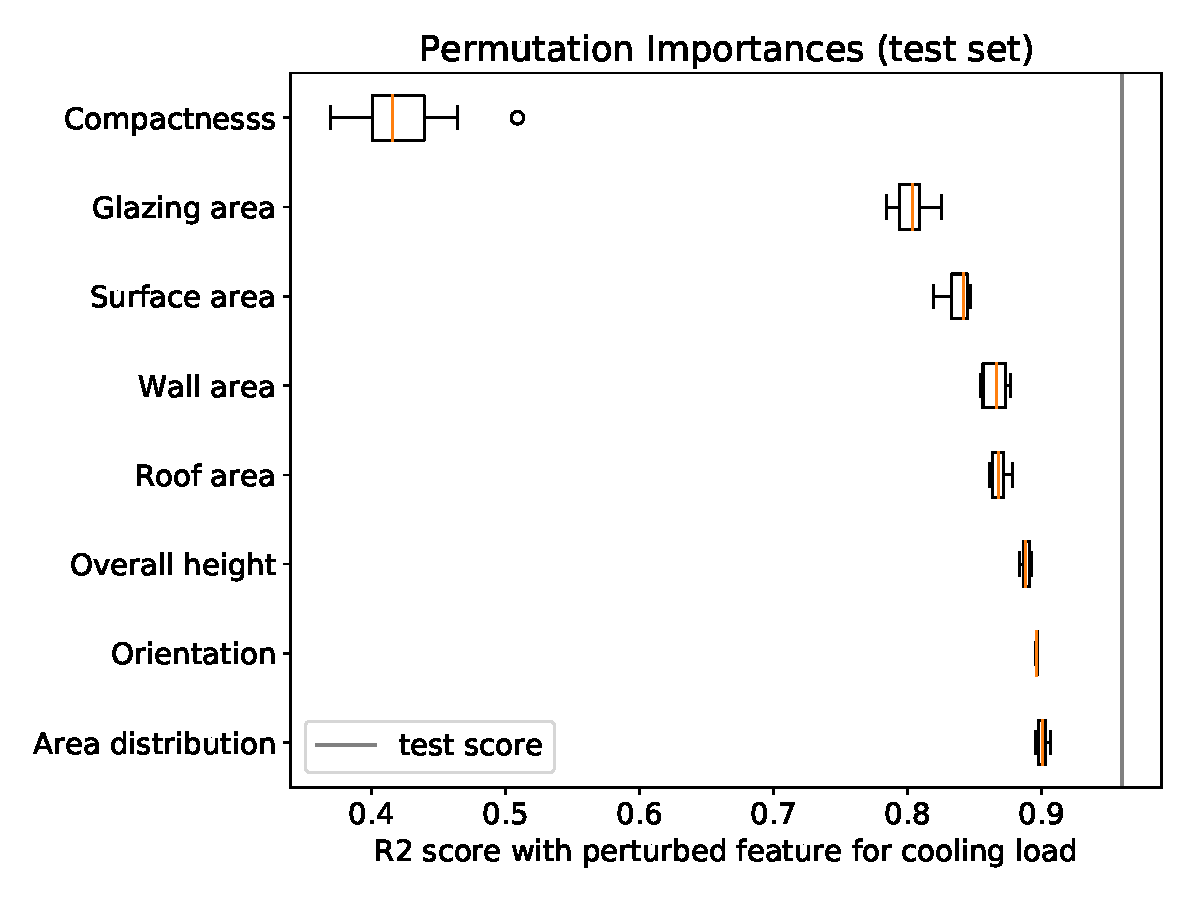
\includegraphics[scale=0.38]{../../figures/Y2_gfi_permutation.pdf}
  \label{fig:permutation_Y2} }
\caption{Global feature importance: permutation test} 
\end{figure}


\begin{figure}[!bht]
\centering     \captionsetup{font=footnotesize, width=.6\textwidth}
\subfigure[Shap global feature importance for heating load]{
  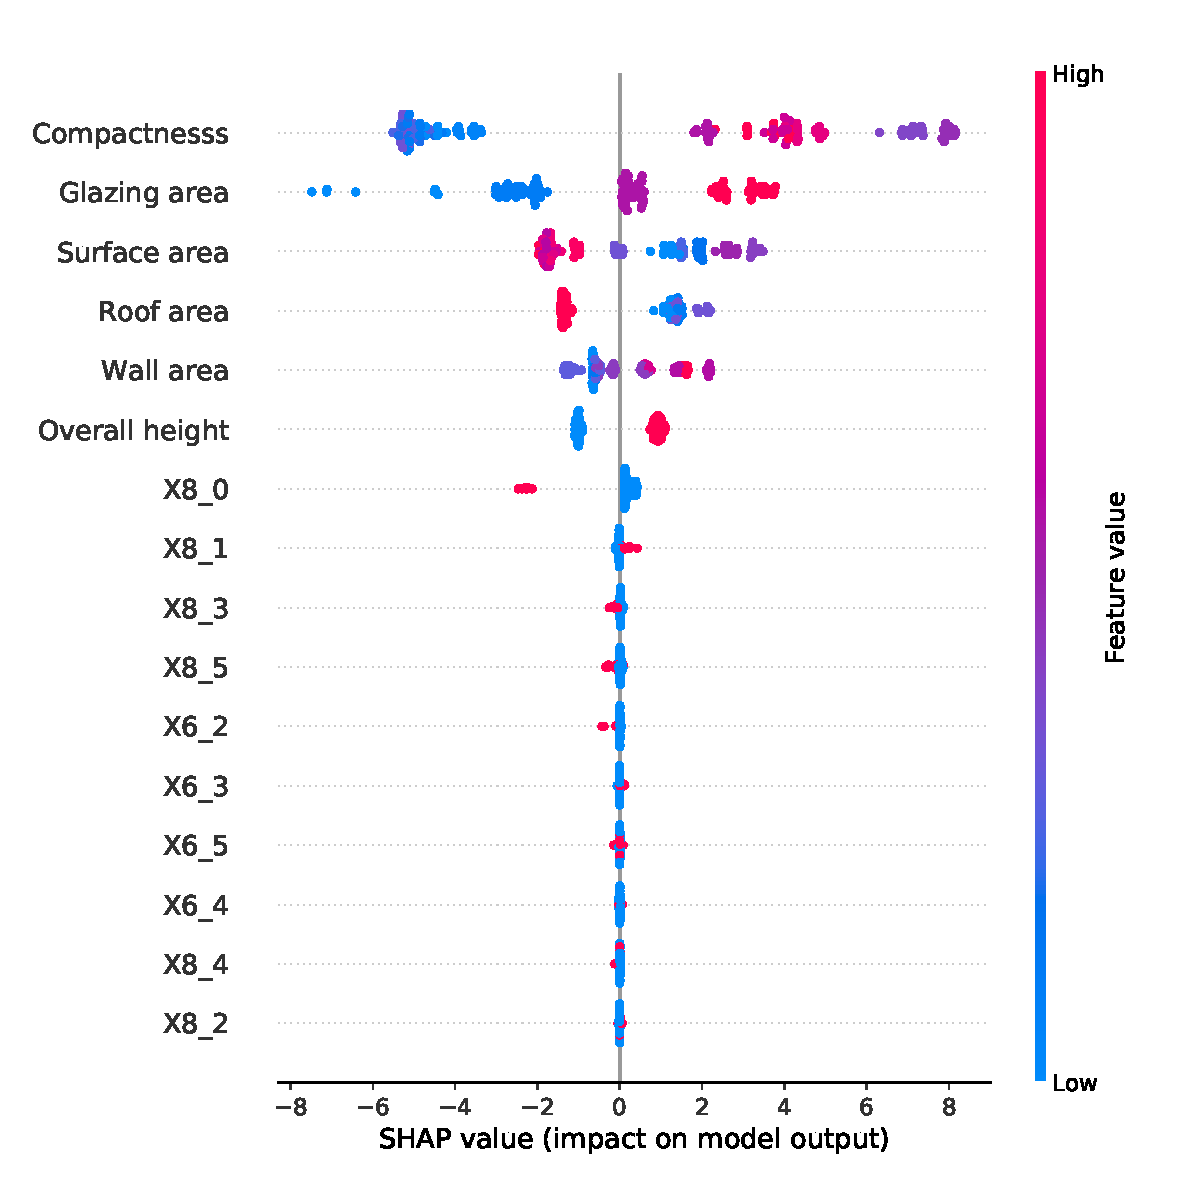
\includegraphics[scale=0.38]{../../figures/shap_Y1_gfi.pdf}
  \label{fig:shap_Y1}}
% \quad
\subfigure[Shap global feature importance for cooling load]{
  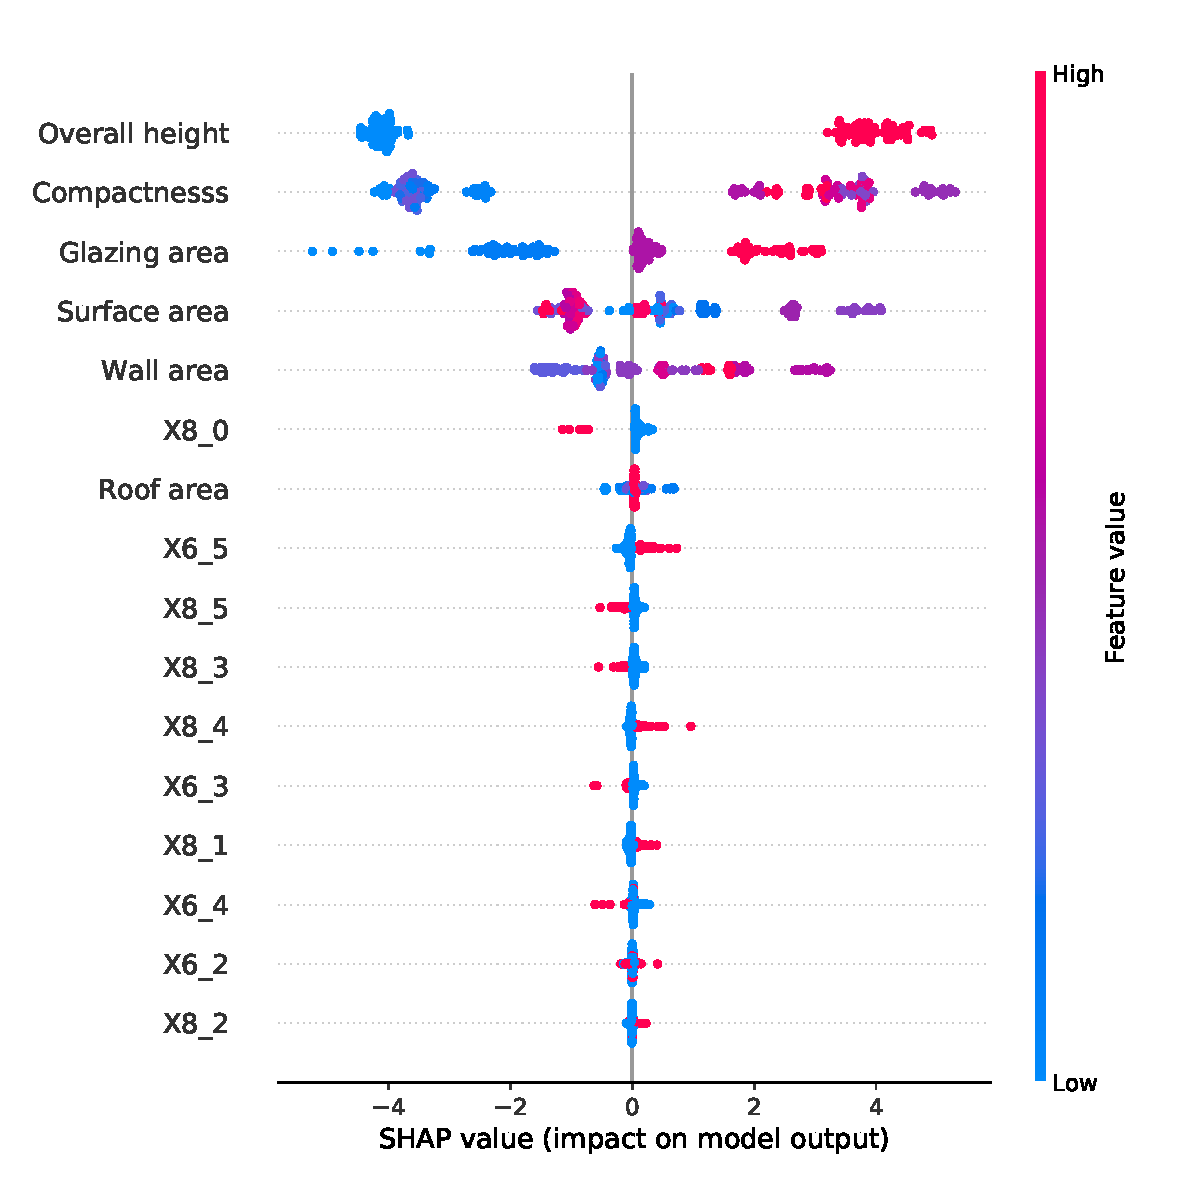
\includegraphics[scale=0.38]{../../figures/shap_Y2_gfi.pdf}
  \label{fig:shap_Y2} }
\caption{Global feature importance: SHAP method} 
\end{figure}


\subsection{Local feature importance \label{subsec:lfi}}
With the help of \textit{SHapley}, I studied the the local feature importance for an example point whose corresponding heating load and cooling load are  $32.57$ and $33.71$, way above the base value of $22.07$. It shows that high compactness and glazing area  contributes the most to a high heating load whereas high overall height and compactness push the cooling load to the right.  

\begin{figure}[!bht]
\centering     \captionsetup{font=footnotesize, width=.6\textwidth}
\subfigure[Shap local feature importance for heating load]{
  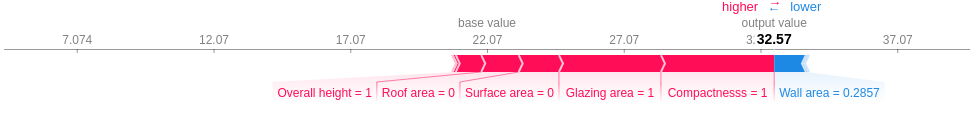
\includegraphics[scale=0.38]{../../figures/Y1_local_importance.png}
  \label{fig:shap_Y1_loc}}
% \quad
\subfigure[Shap local feature importance for cooling load]{
  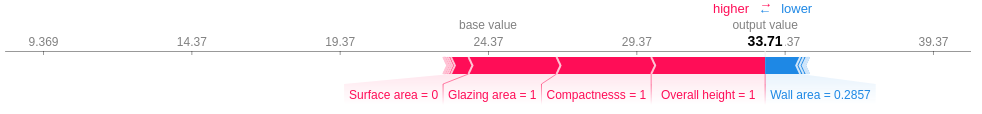
\includegraphics[scale=0.38]{../../figures/Y2_local_importance.png}
  \label{fig:shap_Y2_loc} }
\caption{Local feature importance using shap} 
\end{figure}


\section{Outlook}
We could try other models to improve the performance, such as gradient boosting. We might have missed some important features for the prediction of cooling load, which might be the reason for the poor model performance on it. More formal tests need to be carried out to provide more insights. Also, we can try to tune more parameters, such as activation functions and learning rates for a neural network model.

\section{References}
\begin{enumerate}
\item[1.] The dataset is from \href{https://archive.ics.uci.edu/ml/datasets/Energy+efficiency}{UCI Machine Learning Repository}
\item[2.] A. Tsanas, A. Xifara: 'Accurate quantitative estimation of energy performance of residential buildings using statistical machine learning tools', Energy and Buildings, Vol. 49, pp. 560-567, 2012.
\item[3.] J. Chou, D. Bui: 'Modeling heating and cooling loads by artificial intelligence for energy-efficient building design', Energy and Buildings, Vol. 82, pp. 437-446, 2014.
\end{document}
